\documentclass[a4paper, frenchb, 11pt]{article}

\usepackage[top=2cm, bottom=2cm, left=2cm, right=2cm]{geometry}
\usepackage[utf8]{inputenc}
\usepackage[T1]{fontenc}
\usepackage{babel}

\usepackage{multicol}
\setlength{\columnseprule}{1pt} % separation line between columns

\usepackage{hyperref}
\hypersetup{
	colorlinks=true,	% false: boxed links; true: colored links
	linkcolor=black,	% color of internal links
	urlcolor=blue,		% color of external links
	citecolor=blue
}

\usepackage{graphicx}	% import graphics
\usepackage{wrapfig}	% wrap text around figures
\usepackage{subcaption}

\usepackage{dirtree} % file tree
% Colors
\usepackage[usenames,dvipsnames]{xcolor}

% Colored frame
\usepackage{mdframed}
\usepackage{framed}
\definecolor{shadecolor}{rgb}{0.96,0.96,0.96}
\definecolor{TFFrameColor}{rgb}{0.96,0.96,0.96}
\definecolor{TFTitleColor}{rgb}{0.00,0.00,0.00}
\definecolor{lightred}{rgb}{1,0.96,0.96}
\definecolor{darkred}{rgb}{0.85,0.33,0.31}
\definecolor{lightblue}{HTML}{EBF5FA}
\definecolor{lightblue2}{HTML}{E3F2FA}
\definecolor{darkblue}{HTML}{D2DCE1}
\definecolor{hintbg}{HTML}{FFFAE6}
\definecolor{hintborder}{HTML}{FAE6BE}

% Redefine leftbar envvironment
\newlength{\leftbarwidth}
\setlength{\leftbarwidth}{1pt}
\newlength{\leftbarsep}
\setlength{\leftbarsep}{10pt}

\newcommand*{\leftbarcolorcmd}{\color{leftbarcolor}} % as a command to be more flexible
\colorlet{leftbarcolor}{gray}

\renewenvironment{leftbar}{%
    \def\FrameCommand{{\leftbarcolorcmd{\vrule width \leftbarwidth\relax\hspace {\leftbarsep}}}}%
    \MakeFramed {\advance \hsize -\width \FrameRestore }%
}{%
    \endMakeFramed
}

% Code listings
\usepackage{listings}
\definecolor{dkgreen}{rgb}{0,0.6,0}
\definecolor{steelblue}{rgb}{0.16,0.37,0.58}
\definecolor{gray}{rgb}{0.5,0.5,0.5}
\definecolor{mauve}{rgb}{0.58,0,0.82}
\definecolor{blue}{rgb}{0,0,0.7}
\lstset{
	language=C,
	basicstyle=\scriptsize,
	numbers=left,                   % where to put the line-numbers
  	numberstyle=\tiny\color{gray},
	commentstyle=\color{steelblue},
	stringstyle=\color{BrickRed},
	backgroundcolor=\color{shadecolor},
    keywordstyle=\color{OliveGreen},
	frame=single,                   % adds a frame around the code
 	rulecolor=\color{black},
	emph={},
	emphstyle=\color{mauve},
	morekeywords=[2]{obside@obsideb},
	keywordstyle={\color{black}},
	keywordstyle=[2]{\color{dkgreen}},
	showstringspaces=false,
  	tabsize=4,
	moredelim=[is][\small\ttfamily]{/!}{!/},
	breaklines=true
}

% Title page
\title{
	\textbf{INF-4201B - TP Sockets}\\
}
\date{\today}

\begin{document}
\maketitle
\newpage

\tableofcontents
\newpage

\section{Introduction}
% TODO
% TODO penser à zipper le rapport avec le code source et les envoyer ensemble sur icampus

\subsection{Arborescence}
% TODO arborescence + description en face de chaque fichier/dossier
% TODO alternative : environnement description pour donner un bref résumé des différents fichiers présents et leur utilité
% \dirtree{%
% .1 src.
% .2 exo1.
% .2 exo2.
% .2 exo2_alt.
% .2 exo3.
% .2 exo4.
% .2 exo5.
% .2 file_tools.c/.h.
% .2 http_tools.c/.h.
% .2 socket_tools.c/.h.
% }

\subsection{Outils utilisés}
% TODO parler de netstat, valgrind et cmake

\subsection{Instructions de compilation}
Ci-dessous les instructions pour compiler l'ensemble des exercices. L'utilitaire cmake est nécessaire afin de créer le Makefile.

\begin{mdframed}[backgroundcolor=lightblue, linecolor=darkblue]
	mkdir build\\
	cd build\\
	cmake ..\\
	make
\end{mdframed}

\newpage

\section{Exercice 1}
L'objectif de cet exercice est de créer un client et un serveur communiquant à l'aide de sockets non connectées (\emph{DGRAM\_SOCKETS}). Un des points notables de telles sockets est que si des données sont envoyées, elles n'arrivent pas forcément, et si elles arrivent, elles n'arrivent par forcément dans l'ordre. Elles sont utiles pour avoir une taille de header plus faible (par rapport à des sockets connectées utilisant TCP) et lorsque la perte de quelques paquets n'a pas d'importance.\\

Le client se connecte au serveur, envoie son PID ainsi que le message passé en argument du programme au serveur, puis le serveur envoie au client son PID ainsi que le message précédemment reçu.

\subsection{Client}
Du côté du client, nous souhaitons tout d'abord récupérer l'adresse du serveur à l'aide de son nom (e.g. localhost $\rightarrow$ 127.0.0.1) grâce à la fonction \emph{gethostbyname()}. Une fois cela fait, nous créons la datagram socket.\\

\begin{mdframed}[backgroundcolor=hintbg, linecolor=hintborder]
La fonction \emph{gethostbyname()} est dépréciée, la page de manuel de la fonction conseille d'utiliser \emph{getaddrinfo()} à la place. \emph{gethostbyname()} sera principalement utilisée dans ce TP, ayant commencé à travailler avec. Nous aurons cependant l'occasion de voir l'utilisation de \emph{getaddrinfo()} dans l'exercice 2, deux versions du client ayant été développées.
\end{mdframed}

\begin{mdframed}[backgroundcolor=lightblue2, linecolor=darkblue]
Il est à noter que le pointeur vers la structure \emph{hostent} renvoyé par la fonction \emph{gethostbyname()} ne doit pas être libéré. Celui-ci peut pointer vers des données statiques.

%\begin{mdframed}[backgroundcolor=hintbg, linecolor=hintborder]
\begin{mdframed}[backgroundcolor=lightblue, linecolor=darkblue]
	\textbf{gethostbyname(3) man page} :\\ % TODO http://man7.org/linux/man-pages/man3/gethostbyname.3.html
	``The functions gethostbyname() and gethostbyaddr() may  return  pointers to  static  data, which may be overwritten by later calls.''
\end{mdframed}
\begin{mdframed}[backgroundcolor=lightblue, linecolor=darkblue]
	\noindent\textbf{MSDN hostent structure} :\\ % TODO http://msdn.microsoft.com/en-us/library/windows/desktop/ms738552%28v=vs.85%29.aspx
	``An application should never attempt to modify this structure or to free any of its components.''
\end{mdframed}
\end{mdframed}
\

Nous souhaitons pouvoir envoyer un message au serveur à l'aide de la socket précédemment créée. Pour cela, nous devons utiliser la fonction \emph{sendto} prenant entre autres en paramètre un pointeur vers une structure \emph{sockaddr}. Pour être plus spécifique, nous allons remplir les champs d'une structure \emph{sockaddr\_in} qui est spécifique au protocole IPv4. Cette dernière va permettre d'indiquer à qui envoyer le message. Toutes les informations pour remplir cette structure sont disponibles: la famille d'adresses (ici \emph{AF\_INET} pour IPv4), le port du serveur (récupéré en argument du programme), et l'adresse du serveur (récupérée à l'aide de \emph{gethostbyname()}).

\begin{lstlisting}
struct sockaddr_in dest_addr;

...

dest_addr.sin_family = AF_INET;
dest_addr.sin_port = htons(atoi(argv[2]));
dest_addr.sin_addr = *((struct in_addr*) he->h_addr_list[0]);
memset(dest_addr.sin_zero, 0, sizeof(dest_addr.sin_zero));
\end{lstlisting}
\

La fonction \emph{sendto()} ne garantie pas que le message soit complétement envoyé, la fonction \emph{sendto\_complete} a donc été créée dans le fichier \emph{socket\_tools.c}. Cette fonction fait appel à \emph{sendto()} tant que la taille des données envoyées est inférieure à la taille totale du message à envoyer.

\begin{lstlisting}
int sendto_complete(int sockfd, char* msg, int msg_size,
    const struct sockaddr *dest_addr)
{
    int sent_size = 0;

    while (sent_size < msg_size) {
        int remaining_size = msg_size - sent_size;
        int temp_size = sendto(sockfd, msg + sent_size, remaining_size, 0,
        dest_addr, sizeof(*dest_addr));
        if (temp_size == -1) {
            perror("sendto");
            break;
        }

        sent_size += temp_size;
    }

    return (sent_size != msg_size) ? -1 : 0;
}
\end{lstlisting}
\

Une fois le message complétement envoyé, on souhaite recevoir la réponse du serveur. Pour cela on utilise la fonction \emph{recvfrom\_helper()} définie dans \emph{socket\_tools.c}. Celle-ci exécute l'appel système \emph{recvfrom()} permettant de recevoir des données via des \emph{SOCK\_DGRAM}, puis s'assure que le message se termine par le caractère \textbackslash 0.

\begin{lstlisting}
int recvfrom_helper(int sockfd, char *buffer, int buffer_size, int *recv_size,
    struct sockaddr *src_addr, socklen_t *addrlen)
{
    *recv_size = recvfrom(sockfd, buffer, buffer_size, 0, src_addr, addrlen);
    if (*recv_size == -1) {
        perror("recvfrom");
        return -1;
    }

    // Make sure the received message ends with '\0'.
    if (buffer[*recv_size - 1] != '\0') {
        if (*recv_size == buffer_size) {
            buffer[*recv_size - 1] = '\0';
        }
        else {
            buffer[*recv_size] = '\0';
        }
    }

    return 0;
}
\end{lstlisting}

\subsection{Serveur}
Pour le serveur, la socket est tout d'abord créée puis liée à toute les interfaces et à un port spécifique. La création se fait comme précédemment à l'aide de l'appel système \emph{socket()}, et la liaison se fait à l'aide de \emph{bind()} et d'une structure \emph{sockaddr\_in}. Le port passé en argument du programme est utilisé pour le champ \emph{sin\_port} de la structure, et INADDR\_ANY est passé au champ \emph{sin\_addr.s\_addr}. Cette constante indique que la socket est liée à toutes les interfaces locales. \cite{cite:cmu_edu_inaddr_any} \cite{cite:man_ip}

\begin{mdframed}[backgroundcolor=lightblue, linecolor=darkblue]
\textbf{ip(7) man page :}\\
``When INADDR\_ANY is specified in the bind call, the  socket will be bound to all local interfaces.''
\end{mdframed}

\begin{mdframed}[backgroundcolor=hintbg, linecolor=hintborder]
INADDR\_ANY est représenté par l'adresse \emph{0.0.0.0}, et vaut donc \emph{0x000000} en représentation hexadécimale. Passer cette constante à la fonction \emph{htonl()} n'est donc pas utile, puisque sa valeur hexadécimale est la même en big-endian et en little-endian.
\end{mdframed}
\newpage

\begin{lstlisting}
// Create socket (IPv4, connectionless, UDP)
sockfd = socket(AF_INET, SOCK_DGRAM, 0);
if (sockfd == -1) {
    perror("server - socket init");
    return EXIT_FAILURE;
}

// fill serv_addr
serv_addr.sin_family = AF_INET;
serv_addr.sin_port = htons(atoi(argv[1]));
serv_addr.sin_addr.s_addr = INADDR_ANY;
memset(serv_addr.sin_zero, 0, sizeof(serv_addr.sin_zero));

// bind socket to all local interfaces on the port specified in argument
status = bind(sockfd, (struct sockaddr *) &serv_addr, sizeof(serv_addr));
if (status == -1) {
    perror("server - bind");
    return EXIT_FAILURE;
}
\end{lstlisting}
\

Une fois la socket initialisée, le principe est similaire à celui du client. Des données sont tout d'abord reçues d'un client à l'aide de \emph{recvfrom\_helper}, puis le message est traité afin de remplacer le PID du client par celui du serveur, et enfin le message ainsi modifié est envoyé au client à l'aide de \emph{sendto\_complete}. Ces étapes sont effectuées dans une boucle afin de pouvoir traiter les messages de plusieurs clients.

\subsection{Exemple d'exécution}
\begin{figure}[h!]
	\centering
	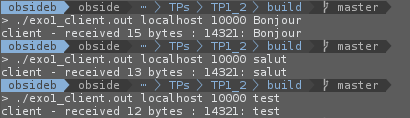
\includegraphics[width=0.8\textwidth]{screenshots/ex1_client.png}
	\caption{exo1\_client.out}
\end{figure}

\begin{figure}[h!]
	\centering
	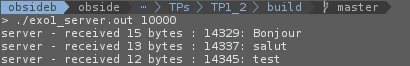
\includegraphics[width=0.8\textwidth]{screenshots/ex1_server.png}
	\caption{exo1\_server.out}
\end{figure}

\newpage

\section{Exercice 2}
Le but de cet exercice est de créer un serveur permettant d'afficher ce qu'un client s'y étant connecté lui a envoyé. Ce serveur nous permettra entre autres de voir la syntaxe d'une requête HTTP GET en connectant un navigateur web sur l'adresse et le port du serveur.

\subsection{Client}
Cela n'était pas demandé dans la consigne, mais un client a tout d'abord été créé. Les fonctions écrites ici nous servirons de nouveau par la suite, notamment celle nous permettant d'initialiser une stream socket du côté d'un client.\\

Nous initialisons tout d'abord la stream socket (socket connectée) soit à l'aide de la fonction \emph{init\_stream\_client\_socket()}, soit à l'aide de la fonction \emph{init\_stream\_client\_socket\_alt()}. Ces fonctions définies dans le fichier \emph{socket\_tools.c} servent à initialiser une socket permettant de se connecter à un serveur en utilisant \emph{gethostbyname()} pour la première, et en utilisant \emph{getaddrinfo()} pour la seconde. Celles-ci seront détaillées par la suite. Une fois l'initialisation de la socket effectuée, les caractères écrits sur l'entrée standard sont envoyés un par un au serveur via la socket. La lecture de caractères s'arrête lorsque le caractère EOF (ctrl + d) est tapé.

\begin{lstlisting}
...

sockfd = init_stream_client_socket(argv[1], atoi(argv[2]));

do {
    int sent_size;

    c = getchar();
    sent_size = send(sockfd, &c, 1, 0);
    if (sent_size == -1) {
        perror("client - send");
    }
} while (c != EOF);

...
\end{lstlisting}

\subsubsection{init\_stream\_client\_socket - gethostbyname}
L'initialisation de la socket connectée côté client est similaire à l'initialisation de la datagram socket vue à l'exercice précédent : récupération des informations du serveur à l'aide de \emph{gethostbyname()}, création de la socket (avec \emph{SOCK\_STREAM} et non plus \emph{SOCK\_DGRAM}), et remplissage de la structure \emph{sockaddr\_in}. A cela vient se rajouter l'étape de connexion de la socket à l'aide de l'appel système \emph{connect()} qui prend en paramètres le descripteur de fichier de la socket, l'adresse de la structure précédemment remplie, et sa taille.\\

\begin{lstlisting}
int init_stream_client_socket(const char* hostname, int port) {
    int sockfd, status;
    struct hostent *he;
    struct sockaddr_in dest_addr;

    // Retrieve server information
    he = gethostbyname(hostname);
    if (he == NULL) {
        perror("client - gethostbyname");
        exit(EXIT_FAILURE);
    }

    // Create socket (IPv4, connected, TCP)
    sockfd = socket(AF_INET, SOCK_STREAM, 0);
    if (sockfd == -1) {
        perror("client - socket init");
        exit(EXIT_FAILURE);
    }

    // Fill dest_addr
    dest_addr.sin_family = AF_INET;
    dest_addr.sin_port = htons(port);
    dest_addr.sin_addr = *((struct in_addr*) he->h_addr_list[0]);
    memset(dest_addr.sin_zero, 0, sizeof(dest_addr.sin_zero));

    // Connect the socket
    status = connect(sockfd, (struct sockaddr*) &dest_addr, sizeof(dest_addr));
    if (status == -1) {
        perror("client - connect");
        exit(EXIT_FAILURE);
    }

    return sockfd;
}
\end{lstlisting}

\subsubsection{init\_stream\_client\_socket\_alt - getaddrinfo}
Comme précisé précédemment, l'utilisation de \emph{getaddrinfo()} est aujourd'hui préférée par rapport à \emph{gethostbyname()}. Une alternative à la fonction précédente (initialisation d'une stream socket du côté client) utilisant \emph{getaddrinfo()} a donc été écrite. \emph{getaddrinfo()} possède plusieurs avantage, le premier étant qu'elle fonctionne pour les protocoles IPv4 et IPv6, et le second étant qu'elle permet d'éviter l'étape de remplissage de la structure \emph{sockaddr}, celle-ci est en effet automatiquement remplie. Le premier paramètre est le nom de l'hôte ou son adresse IP, le second est le numéro de port, et le troisième est une structure \emph{addrinfo} qui va permettre de sélectionner les résultats qui nous intéressent. Enfin, le quatrième est une liste de résultats (liste d'\emph{addrinfo}) qui va être remplie par la fonction.\\

\begin{mdframed}[backgroundcolor=lightblue, linecolor=darkblue]
\noindent \textbf{N.B.} La fonction \emph{getaddrinfo()} ne fait pas partie du standard C99, mais du standard POSIX, il faut donc compiler le programme avec \emph{-D\_POSIX\_SOURCE}.
\end{mdframed}

\begin{lstlisting}
int init_stream_client_socket_alt(const char* hostname, const char *port) {
    int sockfd, status;
    struct addrinfo hints, *res, *tmp;

    memset(&hints, 0, sizeof(hints));
    hints.ai_family = AF_UNSPEC; // IPv4 or IPv6
    hints.ai_socktype = SOCK_STREAM;

    status = getaddrinfo(hostname, port, &hints, &res);
    if (status != 0) {
        fprintf(stderr, "getaddrinfo: %s\n", gai_strerror(status));
        exit(EXIT_FAILURE);
    }

    /* res contains a list of address structures, loop until we successfully
     * connect to the server. */
    for (tmp = res ; tmp != NULL ; tmp = tmp->ai_next) {
        sockfd = socket(tmp->ai_family, tmp->ai_socktype, tmp->ai_protocol);
        if (sockfd == -1) {
            perror("client - socket init");
            continue;
        }

        status = connect(sockfd, tmp->ai_addr, tmp->ai_addrlen);
        if (status == -1) {
            perror("client - connect");
            close(sockfd);
            continue;
        }

        break;
    }

    freeaddrinfo(res);

    if (tmp == NULL) {
        fprintf(stderr, "client - failed to connect to any server\n");
        exit(EXIT_FAILURE);
    }

    return sockfd;
}
\end{lstlisting}

\subsection{Serveur}
Du côté du serveur, la socket est tout d'abord initialisée, une requête de connexion d'un client est attendue et acceptée à l'aide de l'appel système \emph{accept()}, puis on affiche ce qu'a envoyé le client.\\

\begin{lstlisting}
...

sockfd = init_stream_server_socket(atoi(argv[1]));

// Accept one connection request from a client
clientfd = accept(sockfd, NULL, NULL);
if (clientfd == -1) {
    perror("server - accept");
    return EXIT_FAILURE;
}

recv_print_request(clientfd);

...
\end{lstlisting}
\

L'initialisation de la socket est effectuée à l'aide de la fonction \emph{init\_stream\_server\_socket()} définie dans \emph{socket\_tools.c}. Celle-ci prend en paramètre le port sur lequel la socket va être liée. La socket est d'abord créée à l'aide de l'appel système \emph{socket()}. Une structure \emph{sockaddr\_in} est ensuite remplie, celle-ci va nous servir à lier la socket à l'aide de \emph{bind()}. Nous spécifions que nous souhaitons que la socket soit liée à toutes les interfaces (\emph{INADDR\_ANY}), et au port passé en paramètre. Enfin, cette socket jouant un role de serveur, celle-ci doit être marquée comme une socket passive (ou encore socket d'écoute) afin d'accepter des requêtes de connexion par la suite.\\

\begin{lstlisting}
int init_stream_server_socket(int port) {
    int sockfd, status;
    struct sockaddr_in serv_addr;

    // Create socket (IPv4, connected, TCP)
    sockfd = socket(AF_INET, SOCK_STREAM, 0);
    if (sockfd == -1) {
        perror("server - socket init");
        exit(EXIT_FAILURE);
    }

    // Fill serv_addr
    serv_addr.sin_family = AF_INET;
    serv_addr.sin_port = htons(port);
    serv_addr.sin_addr.s_addr = INADDR_ANY;
    memset(serv_addr.sin_zero, 0, sizeof(serv_addr.sin_zero));

    // Bind socket to all local interfaces on the port specified in argument
    status = bind(sockfd, (struct sockaddr *) &serv_addr, sizeof(serv_addr));
    if (status == -1) {
        perror("server - bind");
        exit(EXIT_FAILURE);
    }

    // Passive (listening) socket
    status = listen(sockfd, 1);
    if (status == -1) {
        perror("server - listen");
        exit(EXIT_FAILURE);
    }

    return sockfd;
}
\end{lstlisting}
\

Enfin, on reçoit les messages envoyés par le client à l'aide de \emph{read()} et on les affiche jusqu'à ce qu'il n'y ait plus rien à lire ou que {\textbackslash r \textbackslash n \textbackslash r \textbackslash n} (indication de fin d'une requête HTTP) soit lu. Cette dernière étape est réalisée par la fonction \emph{recv\_print\_request} définie dans le fichier \emph{http\_tools.c}.

\subsection{Requête HTTP}
On souhaite récupérer la syntaxe d'une requête HTTP à l'aide d'un navigateur web, et du serveur écrit pour cet exercice. Pour cela, le serveur est lancé sur un port (e.g 10000) et une requête est lancé depuis le navigateur à destination de \emph{localhost:10000}. Ci-dessous un exemple de requête reçue.

\begin{figure}[h!]
	\centering
	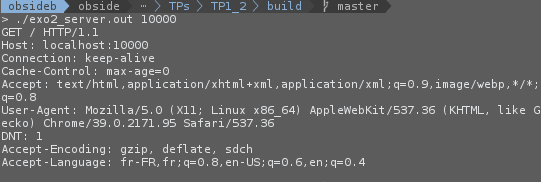
\includegraphics[width=0.8\textwidth]{screenshots/ex2.png}
	\caption{exo2\_server.out - récupération d'une requête HTTP}
\end{figure}

La deux premières lignes de cette requête sont les plus importantes, la première indique que l'on souhaite obtenir la ressource / et que l'on utilise le protocole HTTP/1.1. La seconde ligne indique que la requête est à destination de l'hôte localhost sur le port 10000. Les autres lignes sont optionnelles, et indiquent par exemple de quel navigateur provient la requête, ou encore quels types de fichiers sont acceptés. Les sauts de lignes dans une requête HTTP sont composés d'un retour chariot (\textbackslash r) et d'une nouvelle ligne (\textbackslash n), la dernière ligne étant signalée par deux sauts de ligne (\textbackslash r \textbackslash n \textbackslash r \textbackslash n).

\newpage

\section{Exercice 3}
Le but de cet exercice est de créer un client pouvant se connecter à un serveur web, lui envoyer une requête HTTP, et afficher sa réponse.\\

Le programme utilise trois arguments : le premier est le hostname du serveur, le deuxième le port sur lequel on souhaite se connecter, et le troisième la ressource que l'on souhaite récupérer.\\

La première étape est l'initialisation d'une socket connectée à l'aide de la fonction \emph{init\_stream\_client\_socket} qui a été décrite dans l'exercice précédent. Une fois cette première étape effectuée, nous souhaitons créer et envoyer une requête HTTP au serveur. La création de la requête HTTP se fait à l'aide de la fonction \emph{create\_GET\_request} définie dans \emph{http\_tools.c}.\\

\begin{lstlisting}
char* create_GET_request(const char* host, const char* res, const char* port) {
    char *buf = malloc(BUFFER_LEN);

    int status = snprintf(buf, BUFFER_LEN,
        "GET %s HTTP/1.1\r\n"
        "Host: %s:%s\r\n"
        "Connection: close\r\n"
        "Accept: text/html\r\n\r\n",
        res, host, port
    );

    if(status < 0) {
        free(buf);
        return NULL;
    }

    return buf;
}
\end{lstlisting}
\

La ligne \emph{Connection: close} a été spécifiée afin que l'appel système read qui sera utilisé par la suite puisse retourner 0 lorsqu'il n'y a plus rien à recevoir de la part du serveur. Par défaut, \emph{Connection: Keep-Alive} est utilisé ce qui empêche le dernier read de retourner car la connexion n'a pas été fermée.\\

Une fois la requête créée, on l'envoie à l'aide de \emph{send\_complete()} (similaire à \emph{sendto\_complete()}, mais utilisant \emph{send()} à la place de \emph{sendto()}). On récupère ensuite la réponse à l'aide de \emph{recv\_print()} définie dans \emph{socket\_tools.c} qui effectue des appels à \emph{read()} tant que la taille reçue n'est pas égale à 0 (0 étant retourné lorsqu'il n'y a plus rien à recevoir).\\

\begin{lstlisting}
int recv_print(int sockfd) {
    int recv_size;
    char buf[BUFFER_LEN];

    do {
        recv_size = read(sockfd, buf, BUFFER_LEN - 1);
        if (recv_size == -1) {
            perror("read");
            break;
        }

        if (recv_size != 0) {
            buf[recv_size] = '\0';
            printf("%s", buf);
        }
    } while(recv_size != 0);

    return recv_size;
}
\end{lstlisting}
\newpage

\subsection{Exemple d'exécution}
\begin{figure}[h!]
	\centering
	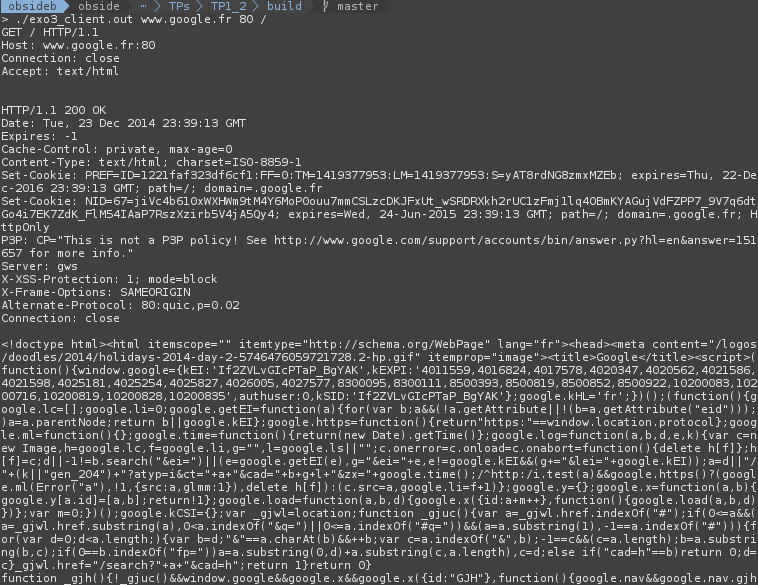
\includegraphics[width=1.0\textwidth]{screenshots/ex3.png}
	\caption{exo3\_client.out}
\end{figure}

\newpage

\section{Exercice 4}
L'objectif de cet exercice est de créer un serveur web répondant aux requêtes HTTP sur un premier port, et renvoyant son fichier de log au client se connectant sur le second port. De nouvelles entrées sont ajoutées dans le fichier de log à chaque fois qu'un client effectue une requête sur le premier port.\\

Deux sockets sont tout d'abord initialisées, \emph{sockfd\_http} et \emph{sockfd\_log} à l'aide de \emph{init\_stream\_ server\_socket()} sur deux ports différents.\\

On souhaite ensuite effectuer un traitement différent si les requêtes sont reçues sur la première ou la seconde socket. Pour cela, les forks ou encore les threads auraient pu être utilisés. Une solution plus simple utilisant la fonction \emph{select()} a cependant été retenue. Cette fonction prend en paramètre des sets de descripteurs de fichiers : \emph{readfds}, \emph{writefds} et \emph{exceptfds}. Celui qui nous intéresse est \emph{readfds}, celui-ci étant modifié lorsque \emph{select()} est exécuté pour indiquer quels descripteurs de fichiers ont des données qui peuvent être lues.\\

\begin{mdframed}[backgroundcolor=lightblue, linecolor=darkblue]
Sachant que les sets passés en paramètre à \emph{select()} sont modifiés à chaque exécution, deux sets sont créés : \emph{master} et \emph{readfds}. A chaque itération de la boucle principale, \emph{master} est copié dans \emph{readfds}, et ce dernier est passé en paramètre de \emph{select()}.

\begin{mdframed}[backgroundcolor=lightblue2, linecolor=darkblue]
\textbf{select(2) man page :}\\
``On exit, the sets are modified in place to indicate which file descriptors actually changed status.''
\end{mdframed}
\end{mdframed}
\

S'il y a des données qui peuvent être lues sur la première socket (\emph{sockfd\_http}), alors on accepte la connexion du client à la socket (\emph{accept()}) puis on traite la requête avec la fonction \emph{handle\_GET\_request()}. Celle-ci fait appel à \emph{recv\_res\_GET\_request()} (fichier \emph{http\_tools.c}) qui permet de recevoir une requête HTTP et la parser afin de récupérer le chemin de la ressource que souhaite obtenir le client. Une ligne est ensuite ajoutée dans le fichier de log au format \emph{adresse du client - date - ressource souhaitée} à l'aide de \emph{log\_line()}. Enfin, le fichier est envoyé à l'aide de la fonction \emph{sendfile\_HTTP\_helper()} (fichier http\_tools.c).\\

\begin{lstlisting}
int handle_GET_request(int clientfd, struct in_addr client_addr) {
    int status;
    char *path, *res;

    // Retrieve resource
    res = recv_res_GET_request(clientfd);
    if (res == NULL) {
        return -1;
    }

    log_line(client_addr, res);

    if (strcmp(res, "/") == 0) {
        path = DEFAULT_PAGE;
    }
    else {
        path = res + 1; // file path without the leading "/"
    }

    status = sendfile_HTTP_helper(path, clientfd);

    free(res);

    return status;
}
\end{lstlisting}
\

La fonction \emph{sendfile\_HTTP\_helper()} ouvre le fichier demandé, puis envoi une réponse 404 (NOT FOUND) si l'ouverture échoue. Si l'ouverture s'effectue correctement, on envoi une réponse 200 (OK) suivie de l'envoi du fichier avec \emph{fsendfile\_helper()} (fichier file\_tools.c).\\

\begin{lstlisting}
int sendfile_HTTP_helper(char* filepath, int fd_dest) {
    int filefd, status;
    char *content_type, *response;

    /* retrieve the content_type with the file extension (unsafe, but probably
     * sufficient for this exercise). */
    if (strstr(filepath, ".html") != NULL) {
        content_type = TYPE_HTML;
    }
    else if(strstr(filepath, ".txt") != NULL) {
        content_type = TYPE_PLAIN_TEXT;
    } else {
        content_type = TYPE_OCTET_STREAM;
    }

    // Open requested file
    filefd = open(filepath, O_RDONLY);
    if (filefd == -1) {
        perror("open");

        // file not found -> HTTP 404 response
        if (errno == ENOENT) {
            send_complete(fd_dest, HTTP_404_RESPONSE, strlen(HTTP_404_RESPONSE));
        }

        return -1;
    }

    // HTTP 200 response
    response = create_HTTP_200_response(content_type);
    if (response == NULL) {
        close(filefd);
        return -1;
    }

    // Send the HTTP response to the client
    status = send_complete(fd_dest, response, strlen(response));
    free(response);
    if (status == -1) {
        close(filefd);
        return -1;
    }

    // send requested file
    status = fsendfile_helper(filefd, fd_dest);

    close(filefd);

    return status;
}
\end{lstlisting}
\

Si des données peuvent être lues sur la seconde socket (\emph{sockfd\_log}), on accepte également la connexion du client, et on envoi le fichier de log avec la fonction \emph{sendfile\_HTTP\_helper()} décrite précédemment.

\newpage
\subsection{Exemple d'exécution}

\begin{figure}[h!]
	\centering
	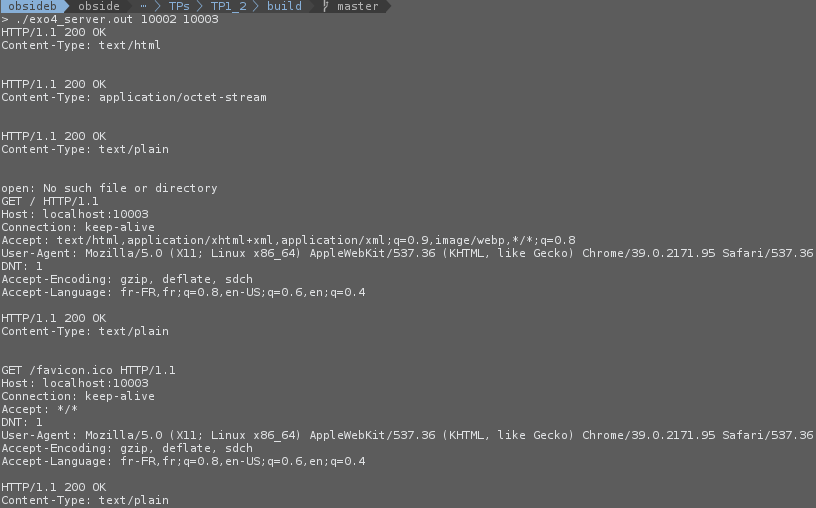
\includegraphics[width=0.9\textwidth]{screenshots/ex4_terminal.png}
	\caption{exo4\_server.out - terminal}
\end{figure}

\begin{figure}[h!]
        \centering
        \begin{subfigure}[b]{0.32\textwidth}
                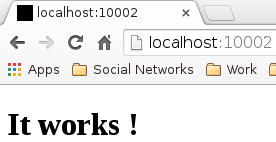
\includegraphics[width=\textwidth]{screenshots/ex4_chrome_index.png}
                \caption{navigateur - index.html}
                \label{fig:ex5_index}
        \end{subfigure}%
        ~
        \begin{subfigure}[b]{0.32\textwidth}
                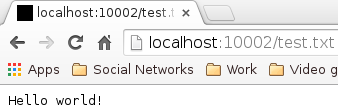
\includegraphics[width=\textwidth]{screenshots/ex4_chrome_test.png}
                \caption{navigateur - test.txt}
                \label{fig:ex5_test}
        \end{subfigure}
        ~
        \begin{subfigure}[b]{0.32\textwidth}
                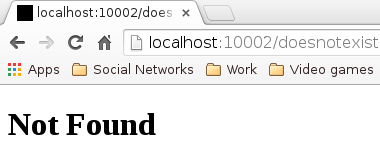
\includegraphics[width=\textwidth]{screenshots/ex4_chrome_doesnotexist.png}
 	            \caption{navigateur - fichier non existant}
                \label{fig:ex5_doesnotexist}
        \end{subfigure}
        \caption{navigateur - requêtes sur le premier port}
\end{figure}

\begin{figure}[h!]
	\centering
	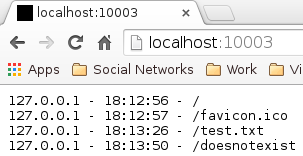
\includegraphics[width=0.4\textwidth]{screenshots/ex4_chrome_log.png}
	\caption{navigateur - requête sur le second port : log}
\end{figure}

\newpage

\section{Exercice 5}
Nous souhaitons à présent envoyer des requêtes en traversant le proxy de l'ESIEE. Pour cela, nous réutilisons l'exercice 3 en passant des paramètres différents à la fonction \emph{create\_GET\_request} de \emph{http\_tools.c}.\\

Le client doit tout d'abord se connecter au proxy de l'ESIEE et non plus directement au serveur web souhaité. Deux constantes \emph{ESIEE\_PROXY\_IP} et \emph{ESIEE\_PROXY\_PORT} ont ainsi été définies dans \emph{http\_tools.h} et sont ensuite utilisées pour se connecter (voir listing ci-dessous).

% FIXME coloration syntaxique
\begin{lstlisting}[caption=Extrait de http\_tools.h]
#define ESIEE_PROXY_IP "147.215.1.189"
#define ESIEE_PROXY_PORT "3128"
\end{lstlisting}
\

Pour qu'une requête HTTP puisse traverser un proxy, il faut que \emph{Request-URI} soit absolue. Nous devons donc passer l'URL complète du site web dans la requête. \emph{Host} quant-à-lui contient l'adresse du proxy.

\begin{lstlisting}[caption=Exemple de requête en passant par le proxy de l'ESIEE, language=bash]
GET http://www.google.com/ HTTP/1.1\r\n
Host: 147.215.1.189:3128\r\n
Connection: close\r\n
Accept: text/html\r\n\r\n
\end{lstlisting}
\

\noindent Ci-dessous un extrait du code de \emph{exo5/client.c} permettant d'effectuer les étapes décrites plus haut.

\begin{lstlisting}
    int sockfd, status;
    char *request;

    if (argc < 2) {
        printf(
            "Missing arguments\n"
            "Usage : %s full_URL\n"
            "Example: %s http://www.google.fr/\n",
            argv[0], argv[0]
        );
        return EXIT_FAILURE;
    }

    sockfd = init_stream_client_socket(ESIEE_PROXY_IP, atoi(ESIEE_PROXY_PORT));

    // Send request
    request = create_GET_request(ESIEE_PROXY_IP, argv[1], ESIEE_PROXY_PORT);
    if (request == NULL) {
        printf("client - could not create the GET request.");
        return EXIT_FAILURE;
    }

    ...
\end{lstlisting}
\newpage

\subsection{Exemple d'exécution}
\begin{figure}[h!]
	\centering
	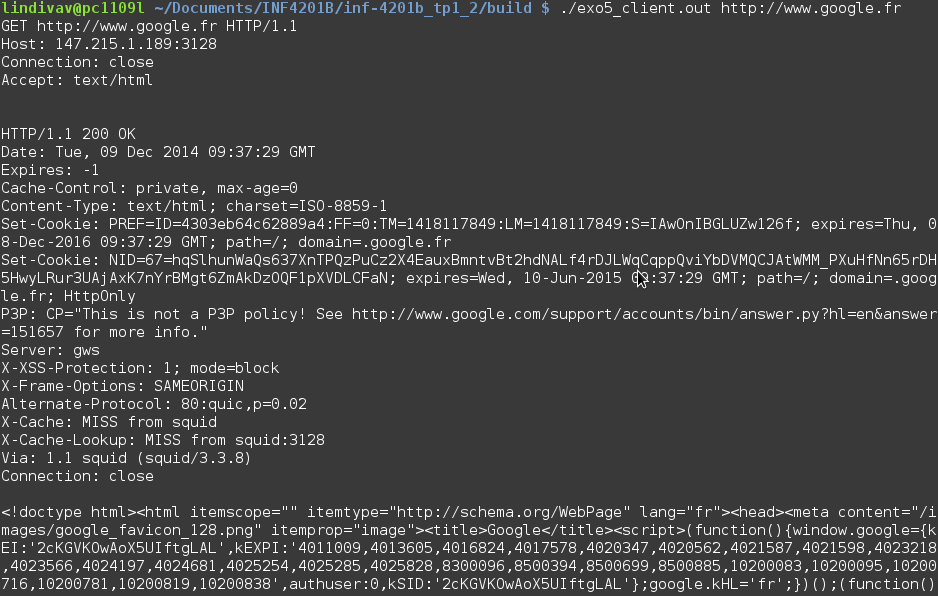
\includegraphics[width=1.0\textwidth]{screenshots/ex5.png}
	\caption{exo5\_client.out}
\end{figure}

\newpage

\renewcommand\refname{Ressources utilisées} % TODO mise en forme
\begin{thebibliography}{5} % TODO
\bibitem{cite:cmake} \emph{CMake}, \href{http://www.cmake.org/}{http://www.cmake.org/}

\bibitem{cite:cmu_edu_inaddr_any} \emph{The IP address INADDR\_ANY}, \href{https://www.cs.cmu.edu/~srini/15-441/F01.full/www/assignments/P2/htmlsim_split/node18.html}{https://www.cs.cmu.edu/~srini/15-441/F01.full/www/assignments/P2/htmlsim\_split/node18.html}

\bibitem{cite:man_ip} \emph{Linux Programmer's Manual - IP(7)}, \href{http://man7.org/linux/man-pages/man7/ip.7.html}{http://man7.org/linux/man-pages/man7/ip.7.html}
% * <http://www.jmarshall.com/easy/http/>
% * <https://github.com/Zintinio/HappyHTTP/blob/master/happyhttp.cpp>
% * <http://stackoverflow.com/questions/11208299/http-get-request-using-c-without-libcurl>
% * <http://www.binarytides.com/receive-full-data-with-recv-socket-function-in-c/>
% * Beej's guide
% * <http://www.binarytides.com/receive-full-data-with-recv-socket-function-in-c/>
% * <http://stackoverflow.com/questions/20922571/server-program-that-listens-on-two-different-socket-interfaces>
\end{thebibliography}

\end{document}
